\documentclass[../mathNotesPreamble]{subfiles}

\begin{document}
%  \relscale{1.4} %TODO
  \section{4.1: Linear Inequalities in Two Variables}

  \subfile{HarMathAp12_prop_of_ineq}
  \pagebreak

  \noindent\textbf{One Linear Inequality in Two Variables}

  \begin{defn*}
      Consider the inequality $y<x$:\\
      The line created by this inequality divides the $xy$-plane into two \textbf{half-planes}. We can determine which half-plane is the solution region by selecting any point \emph{not on the line} as a \textbf{test point}.
  \end{defn*}
  \begin{center}
    \begin{tikzpicture}[declare function={
      f(\x)=\x; xmin=-6.75; xmax=6.75;}]
      \begin{axis}[
        grid=both, %major,minor
        grid style={line width=0.3pt, draw=gray!60},
        major grid style={line width=0.375pt, draw=gray!75},
        axis lines=center,
        axis line style={black,->},
        xmin=xmin, xmax=xmax,
        ymin=xmin,
        ticklabel style={font=\footnotesize,inner sep=0.5pt,fill=white,opacity=0.5, text opacity=1},
        xlabel=$x$, xlabel style={at={(ticklabel* cs:1)},anchor=north west},
        ylabel=$y$, ylabel style={at={(ticklabel* cs:1)},anchor=south west},
        every axis plot/.append style={line width=0.95pt, color=lander_blue, samples=255, domain=xmin:xmax},]
        \addplot[<->, dashed, name path=yltx] {f(x)};
        \addplot[draw=none, name path=negten] {-10};
        \addplot[lander_blue!50,opacity=0.6] fill between[of=yltx and negten];
        \addplot[soldot] coordinates{(2,0)} node[above right, fill=white, yshift=2.5pt, inner sep=2.5pt, opacity=0.65, text opacity=1.0, text=black, rounded corners] {$(2,0)$};
        \node[fill=white, inner sep=2.5pt, opacity=0.65, text opacity=1.0, text=black, rounded corners] at (4,-4) {$y<x$};
        \node[fill=white, inner sep=2.5pt, opacity=0.65, text opacity=1.0, text=black, rounded corners] at (-4,4) {$y>x$};

      \end{axis}
    \end{tikzpicture}
  \end{center}
  \vspace*{\stretch{1}}

  \noindent
  \begin{minipage}[t]{0.5\linewidth}
    \begin{ex*}
      Graph the inequality $3x-2y\leq 6$
    \end{ex*}
  \end{minipage}\hspace*{\stretch{1}}%
  \begin{minipage}[t]{0.425\linewidth}\
    \begin{flushright}
      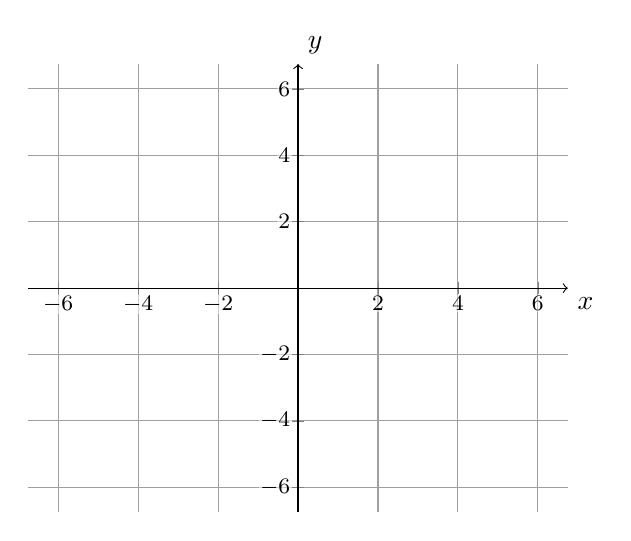
\begin{tikzpicture}[declare function={
        f(\x)=\x; xmin=-6.75; xmax=6.75;}]
        \begin{axis}[
          grid=both, %major,minor
          grid style={line width=0.3pt, draw=gray!60},
          major grid style={line width=0.375pt, draw=gray!75},
          axis lines=center,
          axis line style={black,->},
          xmin=xmin, xmax=xmax,
          ymin=xmin, ymax=xmax,
          ticklabel style={font=\footnotesize,inner sep=0.5pt,fill=white,opacity=0.5, text opacity=1},
          xlabel=$x$, xlabel style={at={(ticklabel* cs:1)},anchor=north west},
          ylabel=$y$, ylabel style={at={(ticklabel* cs:1)},anchor=south west},
          every axis plot/.append style={line width=0.95pt, color=lander_blue, samples=255, domain=xmin:xmax},]
        \end{axis}
      \end{tikzpicture}
    \end{flushright}
  \end{minipage}
  \pagebreak

  \begin{defn*}
    A \textbf{system of inequalities} has two or more inequalities in two or more variables. The solution of the system is the intersection of the individual solution sets.
  \end{defn*}

  \noindent
  \begin{minipage}[t]{0.5\linewidth}
    \begin{ex*}
      \begin{alignat*}{2}
%        r&l&r&l\\
        3x&-&2y&\geq 4\\
        x&+&y&-3>0
      \end{alignat*}
    \end{ex*}
  \end{minipage}\hspace*{\stretch{1}}%
  \begin{minipage}[t]{0.425\linewidth}\
    \begin{flushright}
      \begin{tikzpicture}[declare function={
        xmin=-2.25; xmax=4.5;
        f(\x)=3*\x/2-2; g(\x)=-\x+3;}]
        \begin{axis}[
          grid=both, %major,minor
          grid style={line width=0.3pt, draw=gray!35},
          major grid style={line width=0.375pt, draw=gray!75},
          axis lines=center,
          axis line style={black,->},
          xmin=xmin, xmax=xmax,
          ymin=-2.75, ymax=4.75,
          minor y tick num=1,
          ticklabel style={font=\footnotesize,inner sep=0.5pt,fill=white,opacity=0.5, text opacity=1},
          xlabel=$x$, xlabel style={at={(ticklabel* cs:1)},anchor=north west},
          ylabel=$y$, ylabel style={at={(ticklabel* cs:1)},anchor=south west},
          every axis plot/.append style={line width=0.95pt, color=lander_blue, samples=255}]
          \addplot[<->, name path=fx, domain=-0.5:4.5] {f(x)};
          \addplot[<->, dashed, name path=gx, domain=-1.75:4.55] {g(x)};
          \addplot[lander_blue!50,opacity=0.6] fill between[of=fx and gx, soft clip={domain=2:xmax}];
        \end{axis}
      \end{tikzpicture}
    \end{flushright}
  \end{minipage}
  \vspace*{\stretch{1}}

  \noindent
  \begin{minipage}[t]{0.5\linewidth}
    \begin{ex*}
      Graph the solution of the system
    \begin{alignat*}{3}
%      r&l&r&l&r&l\\
      3x&-&4y&\leq& 12\\
      2x&+&5y&>& 10\\
      x&-&8y&\geq& -16
    \end{alignat*}
  \end{ex*}
  \end{minipage}\hspace*{\stretch{1}}%
  \begin{minipage}[t]{0.425\linewidth}\
    \begin{flushright}
      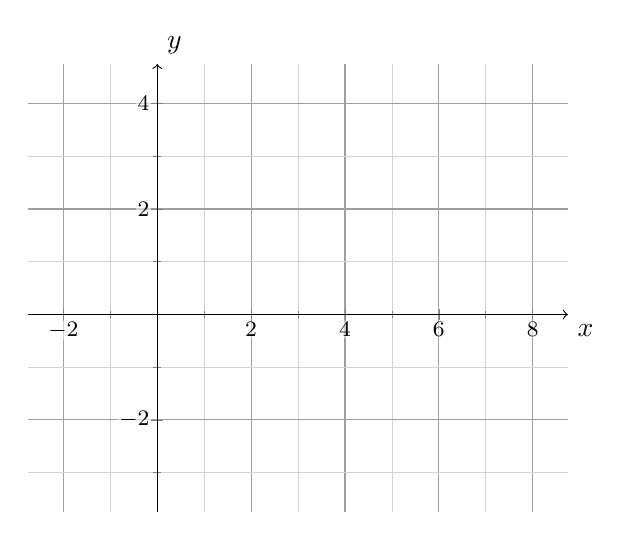
\begin{tikzpicture}
        \begin{axis}[
          grid=both, %major,minor
          grid style={line width=0.3pt, draw=gray!35},
          major grid style={line width=0.375pt, draw=gray!75},
          axis lines=center,
          axis line style={black,->},
          xmin=-2.75, xmax=8.75, minor x tick num=1,
          ymin=-3.75, ymax=4.75, minor y tick num=1,
          ticklabel style={font=\footnotesize,inner sep=0.5pt,fill=white,opacity=0.5, text opacity=1},
          xlabel=$x$, xlabel style={at={(ticklabel* cs:1)},anchor=north west},
          ylabel=$y$, ylabel style={at={(ticklabel* cs:1)},anchor=south west},
          every axis plot/.append style={line width=0.95pt, color=lander_blue, samples=255}]
        \end{axis}
      \end{tikzpicture}
    \end{flushright}
  \end{minipage}
  \vspace*{\stretch{1}}
  \pagebreak

  \begin{ex*}
    CDF Appliances has assembly plants in Atlanta and Fort Worth, where the company produces a variety of kitchen appliances, including a 12-cup coffee maker and a cappuccino machine. The following table shows each factory's assembly capabilities for the two products and the numbers needed to fill orders.
    \begin{center}
      \begin{tabular}{@{}lccc@{}}\toprule
        & \textbf{Atlanta}& \textbf{Fort Worth}& \textbf{Needed}\\\midrule
        Coffee maker& 160/hr& 800/hr& At least 64,000\\
        Cappucino machine& 200/hr& 200/hr& At least 40,000\\\bottomrule
      \end{tabular}
    \end{center}
    Write the system of inequalities that describes the number of assembly hours needed at each plant to fill the orders and graph the solution region for the system
  \end{ex*}
  \vspace*{\stretch{1}}
  \begin{flushright}
    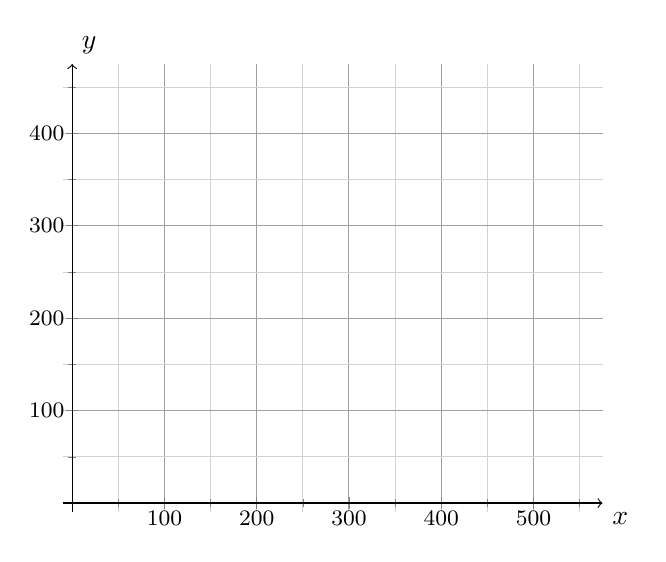
\begin{tikzpicture}
      \begin{axis}[
        grid=both, %major,minor
        grid style={line width=0.3pt, draw=gray!35},
        major grid style={line width=0.375pt, draw=gray!75},
        axis lines=center,
        axis line style={black,->},
        xmin=-10, xmax=575, minor x tick num=1,
        ymin=-10, ymax=475, minor y tick num=1,
        ticklabel style={font=\footnotesize,inner sep=0.5pt,fill=white,opacity=0.5, text opacity=1},
        xlabel=$x$, xlabel style={at={(ticklabel* cs:1)},anchor=north west},
        ylabel=$y$, ylabel style={at={(ticklabel* cs:1)},anchor=south west},
        every axis plot/.append style={line width=0.95pt, color=lander_blue, samples=255}]
      \end{axis}
    \end{tikzpicture}
  \end{flushright}
  \pagebreak

  \begin{ex*}
    A farm co-op has 6000 acres available to plant with corn and soybeans. Each acre of corn requires 9 gallons of fertilizer/herbicide and 3/4 hour of labor to harvest. Each acre of soybeans requires 3 gallons of fertilizer/herbicide and 1 hour of labor to harvest. The co-op has available at most 40,500 gallons of fertilizer/herbicide and at most 5250 hours of labor for harvesting. The number of acres of each crop is limited (constrained) by the available resources: land, fertilizer/herbicide, and labor for harvesting. Write the system of inequalities that describes the constraints and graph the solution region for the system.
  \end{ex*}
  \vspace*{\stretch{1}}
  \begin{flushright}
    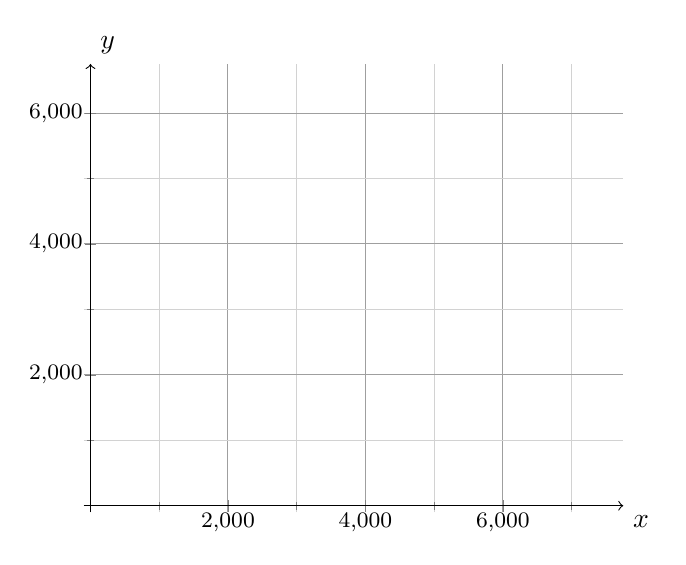
\begin{tikzpicture}
      \begin{axis}[
        grid=both, %major,minor
        grid style={line width=0.3pt, draw=gray!35},
        major grid style={line width=0.375pt, draw=gray!75},
        axis lines=center,
        axis line style={black,->},
        xmin=-100, xmax=7750, minor x tick num=1,
        ymin=-100, ymax=6750, minor y tick num=1,
        ticklabel style={font=\footnotesize,inner sep=0.5pt,fill=white,opacity=0.5, text opacity=1},
        xlabel=$x$, xlabel style={at={(ticklabel* cs:1)},anchor=north west},
        ylabel=$y$, ylabel style={at={(ticklabel* cs:1)},anchor=south west},
        every axis plot/.append style={line width=0.95pt, color=lander_blue, samples=255}]
      \end{axis}
    \end{tikzpicture}
  \end{flushright}
  \pagebreak

  \begin{ex*}
    Graph the solution region for the system
      \begin{alignat*}{3}
%        r&l&r&l&r&l\\
        5x&+&2y&\leq &54\\
        2x&+&4y&\leq &60\\
        &&\mathllap{x\geq0,}\ y& \geq &0
      \end{alignat*}
    Then compute the corners of this region.
  \end{ex*}
  \vspace*{\stretch{1}}
  \begin{flushright}
    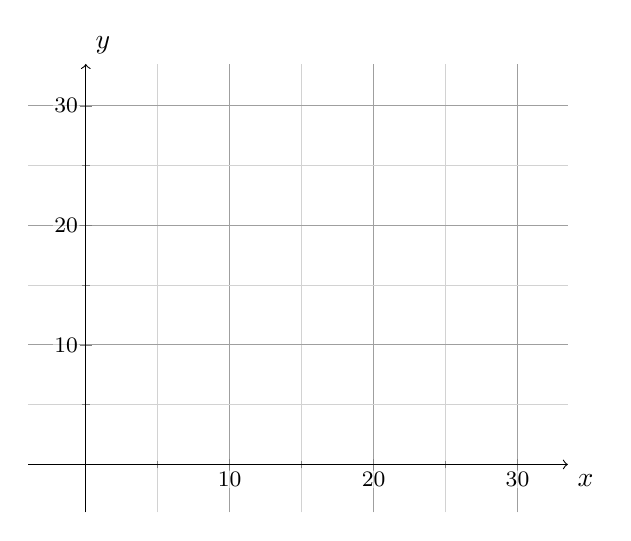
\begin{tikzpicture}
      \begin{axis}[
        grid=both, %major,minor
        grid style={line width=0.3pt, draw=gray!35},
        major grid style={line width=0.375pt, draw=gray!75},
        axis lines=center,
        axis line style={black,->},
        xmin=-4, xmax=33.5, minor x tick num=1,
        ymin=-4, ymax=33.5, minor y tick num=1,
        ticklabel style={font=\footnotesize,inner sep=0.5pt,fill=white,opacity=0.5, text opacity=1},
        xlabel=$x$, xlabel style={at={(ticklabel* cs:1)},anchor=north west},
        ylabel=$y$, ylabel style={at={(ticklabel* cs:1)},anchor=south west},
        every axis plot/.append style={line width=0.95pt, color=lander_blue, samples=255}]
      \end{axis}
    \end{tikzpicture}
  \end{flushright}

  \pagebreak
\end{document}
